% This was adapted from https://github.com/deselaers/latex-beamerposter/blob/master/examples/03/poster.tex


\documentclass{beamer}
\usepackage[orientation=portrait,size=a0,scale=1.4,debug]{beamerposter}
\mode<presentation>{\usetheme{ZH}}
\usepackage{chemformula}
\usepackage[utf8]{inputenc}
\usepackage[german, english]{babel} % required for rendering German special characters
\usepackage{siunitx} %pretty measurement unit rendering
\usepackage{hyperref} %enable hyperlink for urls
\usepackage{ragged2e}
\usepackage[font=scriptsize,justification=justified]{caption}
\usepackage{array,booktabs,tabularx}
\usepackage{lipsum}
\usepackage{blindtext}

% Replacement font for Akzidenz
\usepackage{helvet}

\newcolumntype{Z}{>{\centering\arraybackslash}X} % centered tabularx columns
\sisetup{per=frac,fraction=sfrac}

\title{\huge Template for your posters - Deep Machine Learning}
\author{Student1 Studentsson, Student2 Studentsson}
\institute[Chalmers]{Chalmers University of Technology \\ Electrical Engineering Department}
\date{\today}

% edit this depending on how tall your header is.
\newlength{\columnheight}
\setlength{\columnheight}{104cm}


\begin{document}
\begin{frame}
\begin{columns}
	\begin{column}{.43\textwidth}
		\begin{beamercolorbox}[center]{postercolumn}
			\begin{minipage}{.98\textwidth}  % tweaks the width, makes a new \textwidth
				\parbox[t][\columnheight]{\textwidth}{
					\begin{myblock}{Introduction}
				        This is the template you'll use for your poster. You can add images:
				    
				        \begin{figure}
				            \centering
				            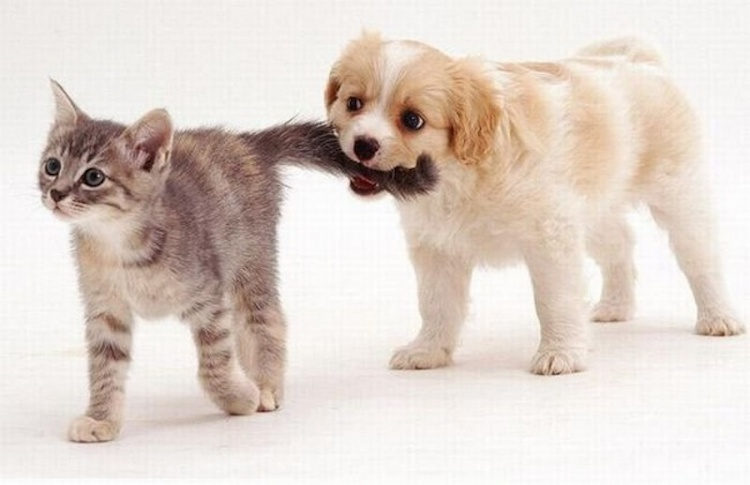
\includegraphics{img/love-is-real-cats-and-dogs-4.jpg}
				            \caption{Very relevant image}
				            \label{fig:my_label}
				        \end{figure}
				        
				        Lists:
				        
				        \begin{itemize}
				            \item List item 1
				            \item List item 2
				            \item List item 3
				            \begin{itemize}
				                \item Sub-list item 1
				                \item Sub-list item 2
				            \end{itemize}
				        \end{itemize}
				        
				        And pretty much anything you can do in \LaTeX{}.
				        
				        
				    \end{myblock}\vfill
					\begin{myblock}{Engagement}
                        Make sure to keep your template engaging. To accomplish this, try to:
                        \begin{itemize}
                            \item Use images and diagrams to attract the reader and illustrate your ideas
                            \item Don't write too much text (like a huge paragraph)
                            \item Make the layout clear and as accessible as possible
                        \end{itemize}
                        
                        For instance, instead of:
                        
                        \begin{figure}
                            \centering
                            \fbox{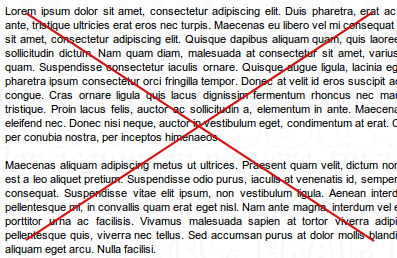
\includegraphics[scale=2]{img/loremipsum_exampletext.png}}
                            \caption{A bad idea for posters...}
                            \label{fig:my_label}
                        \end{figure}
                        
                        Find the main points you want to express and use a list
                        \begin{itemize}
                            \item Lorem
                            \item ipsum
                            \item sit amet
                            \item consectetur
                        \end{itemize}
                        
                        Or even better, use a diagram:
                        
                        \begin{figure}
                            \centering
                            
\includegraphics[scale=2]{img/lorem_ipsum_image.jpg}
                            \caption{Of course, the diagram needs to be useful.}
                            \label{fig:my_label}
                        \end{figure}
                        
					\end{myblock}\vfill
		}\end{minipage}\end{beamercolorbox}
	\end{column}
	\begin{column}{.57\textwidth}
		\begin{beamercolorbox}[center]{postercolumn}
			\begin{minipage}{.98\textwidth} % tweaks the width, makes a new \textwidth
				\parbox[t][\columnheight]{\textwidth}{ 
					\begin{myblock}{Other tips}
    						\begin{itemize}
        						\item Feel free to use equations to illustrate your point
        						
        						\begin{align*} 
            						\sqrt{2} \vee \pi & < \oint_{\infty}^{i} \cosh^{-1} \left(-\infty \right) \,d \Gamma \vee \dots \pm \cosh^{-1} \left( e \Delta \right).
        						\end{align*} 
        						
        						But make sure not to overdo it. Leave the details for your paper.
        						
    					        \item Before you start editing this file, have a clear idea of how you want your poster to look like.
    					        \item Think about who's the target audience. Put yourself in their shoes. Amidst several others, would you stop to read your post?
					    \end{itemize} 
					    
					\end{myblock}\vfill
					\begin{myblock}{Short example}
					    \vspace{1cm}
					    \begin{columns}
					        \begin{column}{0.5\textwidth}
					            \begin{figure}
					                \centering
					                
\includegraphics[scale=0.8]{img/catdog.jpg}
					                \caption{A catdog}
					                \label{fig:my_label}
					            \end{figure}
					        \end{column}
					        
					        \begin{column}{0.5\textwidth}
					            Is this a cat or a dog?
					            \begin{itemize}
					                \item Pretty easy to tell, right?
					                \item Well, maybe not for a computer...
					                \item Imagine you can only see the 1s and 0s. How can a computer solve this?
					            \end{itemize}
					        \end{column}
					    \end{columns}
					    
					    \vspace{1cm}
					    Current best approach
					    \vspace{1cm}
					    \begin{itemize}
					        \item Convolutional neural networks (CNNs)
					        \item Training CNNs requires large amounts of data
					        \item For each data point, we need to know its correct class beforehand
					    \end{itemize}
					    
					    \vspace{1cm}
					    \begin{figure}
					        \centering
					        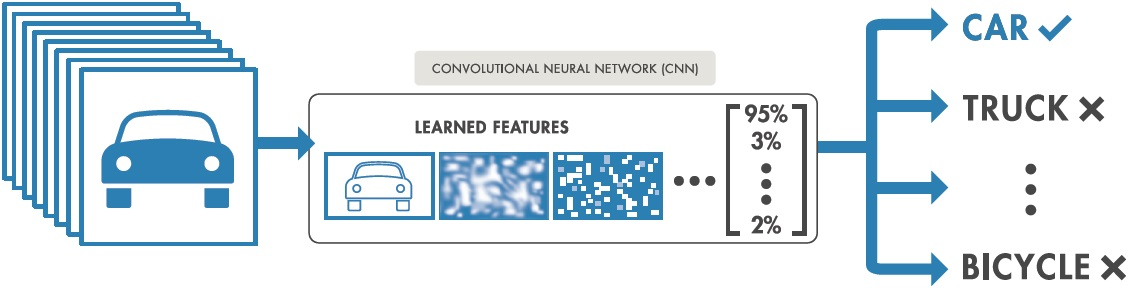
\includegraphics[scale=0.9]{img/cnn.jpg}
					        \caption{CNN framework}
					        \label{fig:my_label}
					    \end{figure}
					    
					    We compare the outputs from the CNN to the desired ones, and adjust its parameterization accordingly, using one of many optimization algorithms.
					    \vspace{1cm}
					    \begin{itemize}
					        \item Used gradient descent\cite{Paivi} for optimization
					        \item Kaggle dataset of Cats vs Dogs \cite{Oegren2008} (25k images of cats and dogs)
					        \item Achieved accuracy of more than 90\% on new images!
					    \end{itemize}
					    					    
					    \begin{figure}
					        \centering
					        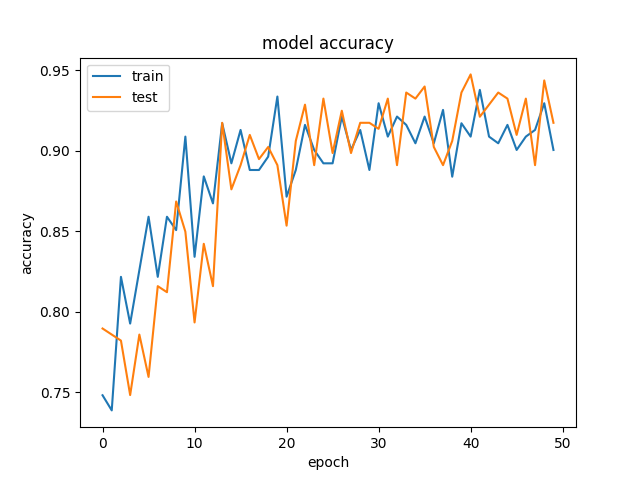
\includegraphics[scale=1.5]{img/accuracy_train.png}
					        \caption{Caption}
					        \label{fig:my_label}
					    \end{figure}
					    
					\end{myblock}
					\begin{myblock}{References}
						\footnotesize
						\bibliographystyle{abbrv}
						\bibliography{./bib}
					\end{myblock}\vfill
		}\end{minipage}\end{beamercolorbox}
	\end{column}
\end{columns}
\end{frame}
\end{document}
